An overall design and architecture was designed in the early sprints of the project.
The server side software is different from the rest of the software made in the project group, as the customers will never actually see it in action, it works perfect if they never notice it is there.
Almost all requirements from our customers concern the user interface and general feel of the apps for the mobile devices. In regards to the server software it is the requirements of the multi project that are of interest,
in particular the oasis group, as their responsibility is to link the rest of the world to us.

The giraf system is designed in such a way that it deploys with two databases: Savannah - our project, a global database for a full deployment unit and Oasis - or localDB, a local database which exists only
on the mobile devices, which has an almost identical schema to the Savannahs database.
Rather than having Oasis query the global database directly, it was decided to implement access to both the databases through a software layer.
The pros and cons of this seemingly redundant software layer was considered, see \autoref{table:proconSoftwareLayers}

\begin{figure}[H]
	\centering
		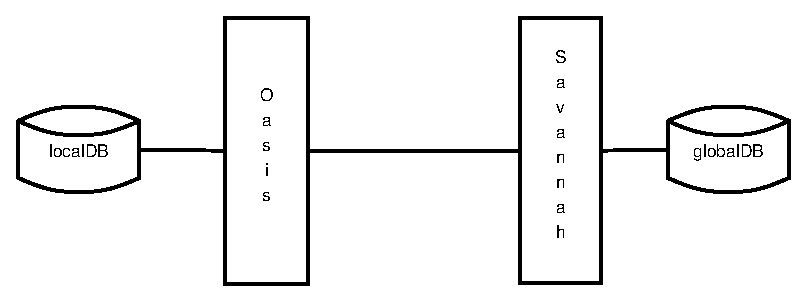
\includegraphics[scale=1]{images/softwareLayers} %FIXME epstopdf package fucker, har ændret noget her
	\caption{Software layers}
	\label{fig:softwareLayers}
\end{figure}

\begin{table}[H]
  \begin{center}
    \begin{tabular}{c|c}
    Pros            &             Cons \\
    \hline
    More flexibilty & higher complexity\\
                    & Lower performance\\
    
    \end{tabular}
    \caption{pros and cons of an extra software layer between the databases}
    \label{table:proconSoftwareLayers}
  \end{center}
\end{table}

Having an extra software layer between the databases means we can alter the global and local databases independently of each other. By providing software with methods for extracting specific
details from Savannah, like full profiles, oasis does not have worry about Savannahs internal database schema. The downside of this is that the complexity inevitably will be higher, and performance
will be lower, the performance issue is not critical though, since the perceived performance of the system will be dominated by the bandwidth of the mobile devices.  

